% English translation of essay/ActPIM_初稿_v3.md, Section III.
\section{Architecture Design}
\label{sec:architecture}

\subsection{System Overview}
\label{sec:architecture-a}

\sys{} is a GPU--LPDDR5X-PIM heterogeneous system for parallel VLA inference; its overall architecture is shown in \todo{system-overview figure}. The GPU executes the VLM as well as the nonlinear operators of the AE, such as normalization and softmax, while the PIM executes the linear operators of the AE and applies RoPE locally.

To let the VLM and the AE execute in parallel, \sys{} partitions memory resources at rank granularity: in each LPDDR5X channel, one DRAM rank serves the memory accesses of the VLM on the GPU, and the other, a PIM rank, executes the AE. The choice of rank granularity follows from the LPDDR memory hierarchy. The channel is the highest level of LPDDR, and the two channels in a package each have independent C/A and DQ interfaces; partitioning by channel would mean that the channels assigned to PIM no longer feed the GPU, halving the bandwidth available to the GPU. The rank, in contrast, is the highest level at which storage and computation can be time-multiplexed: the two ranks of a channel have independent memory arrays selected by their own CS, but share the DQ and C/A buses of the channel. Hence, while the PIM rank computes with the internal bank bandwidth, all channels can still feed the GPU through the DRAM ranks, so that the external transfer bandwidth and the internal compute bandwidth are utilized simultaneously. Going further down to bank-group or bank granularity would require the banks of the same rank to maintain both the normal-access and the PIM-execution states and to handle both classes of commands at the same time, which considerably complicates the control logic. Rank partitioning is therefore the option with the lowest additional overhead. Its cost is that the two ranks contend for the shared DQ bus, which is the problem addressed in the rest of this paper.

Concretely, \sys{} uses eight LPDDR5X-8533 packages (following Micron \todo{verify part number}), each with four dies, two channels, and two ranks, providing 16 independent x16 channels with a peak bandwidth of 273~GB/s.

Each PIM rank contains 4 bank groups (BGs) of 4 banks each. Its compute organization follows the LPDDR5X-PIM published by Samsung~\cite{samsung_lpddr5x_pim}: each bank has one $16\times$ BF16 MAC unit (FP32 accumulation) and one RoPE unit, together with a 1~KiB Input Buffer and a 2~KiB Output Buffer; BG-level and rank-level accumulators aggregate the partial sums level by level. Table~\ref{tab:pim-spec} compares the key specifications with those of the Samsung device.

% User-supplied package-level comparison, 2026-11-17.
% Throughput normalization and AHASD scope assumptions are stated below.
\begin{table}[!t]
\caption{Key Specifications Normalized to Four x16 PIM Dies}
\label{tab:pim-spec}
\centering
\footnotesize
\setlength{\tabcolsep}{2pt}
\begin{tabularx}{\columnwidth}{@{}>{\raggedright\arraybackslash}p{0.135\columnwidth}*{4}{>{\raggedright\arraybackslash}X}@{}}
\toprule
\textbf{Item} & \textbf{\sys{}} & \textbf{LP-Spec~\reviewcite{lp_spec}} & \textbf{AHASD~\reviewcite{ahasd}} & \textbf{Samsung~\reviewcite{samsung_lpddr5x_pim}} \\
\midrule
Interface & LPDDR5X-8533 & LPDDR5 & LPDDR5 & LPDDR5X-9600 \\
Banks & 64 & 64 & 64 & 64 \\
Native type & BF16 & INT8 & INT8 & FP8/INT8 \\
Compute$^{*}$ & 546\,GFLOPS$^{\dagger}$ & 819\,GFLOPS & 205\,GFLOPS$^{\S}$ & 614\,GFLOPS \\
Internal BW & 546\,GB/s$^{\dagger}$ & 410\,GB/s$^{\ddagger}$ & 256\,GB/s$^{\S}$ & 614\,GB/s \\
Input buffer & 64\,KiB & 64\,KiB & 8\,KiB$^{\P}$ & 32\,KiB \\
Output buffer & 128\,KiB & 128\,KiB & 8\,KiB$^{\P}$ & 8\,KiB \\
\bottomrule
\end{tabularx}
\par\vspace{2pt}
\parbox{\columnwidth}{\scriptsize\raggedright
Comparison basis: x64, $4\times$x16 PIM dies.
Each dual-rank x32 \sys{} package uses two PIM dies (32 PIM banks).
$^{*}$BF16-equivalent; 8-bit throughput halved (same datapath width).
$^{\dagger}$One 256-bit access per bank per $t_{\mathrm{CCD\_L}}$ (4\,CK at 1066.7\,MHz), 16 BF16 MAC/access.
$^{\ddagger}$One 256-bit access per bank per 5\,ns.
$^{\S}$Scope not stated in~\reviewcite{ahasd}; compute assumes 102.4\,GOPS per die, BW as reported.
$^{\P}$\texttt{GRF\_A}/\texttt{GRF\_B}, $8\times256$\,b each per PIM block (1 per 2 banks), from the open-source simulator of~\reviewcite{ahasd}.\\[2pt]
\textit{Timing.} \sys{} (CK):
$t_{\mathrm{FAW}}{=}16$, $t_{\mathrm{RAS}}{=}45$, $t_{\mathrm{RCD,RD}}{=}20$, $t_{\mathrm{RPpb}}{=}20$, $t_{\mathrm{CCD\_L}}{=}4$.
LP-Spec: $t_{\mathrm{RP}}{=}15$, $t_{\mathrm{RCD}}{=}15$, $t_{\mathrm{RAS}}{=}34$, $t_{\mathrm{RRD}}{=}4$, $t_{\mathrm{FAW}}{=}16$, $t_{\mathrm{CCD}}{=}4$.
AHASD: $t_{\mathrm{RP}}{=}32$, $t_{\mathrm{RCD}}{=}32$, $t_{\mathrm{RAS}}{=}64$, $t_{\mathrm{FAW}}{=}64$, $t_{\mathrm{CCD\_L}}{=}6$.
Samsung: not disclosed.}
\end{table}


On top of this structure, \sys{} mitigates shared-bus contention in two ways: by organizing the timing of transfers and by reducing their volume. At the microarchitecture level, \sys{} adds a path from the Row Buffer to the Input Buffer. Inputs are first written in bulk into the DRAM of the PIM rank and then broadcast to all banks within the rank. This keeps the tile-by-tile input feeding of the compute phase inside the rank and creates contiguous access windows for the GPU (Section~\ref{sec:architecture-b}); the corresponding commands are encoded in a JEDEC-compatible way (Section~\ref{sec:architecture-c}). At the dataflow level, \sys{} adopts a token-wise layout designed for the shared bus and applies RoPE inside the banks, reducing the data that must cross the DQ bus (Section~\ref{sec:dataflow-a}). Finally, GPU--PIM co-scheduling partitions DQ ownership between the two at kernel granularity, combining these mechanisms into parallel execution (Section~\ref{sec:dataflow-b}).

\subsection{Input-Preloading Microarchitecture}
\label{sec:architecture-b}

\begin{figure*}[!t]
\centering
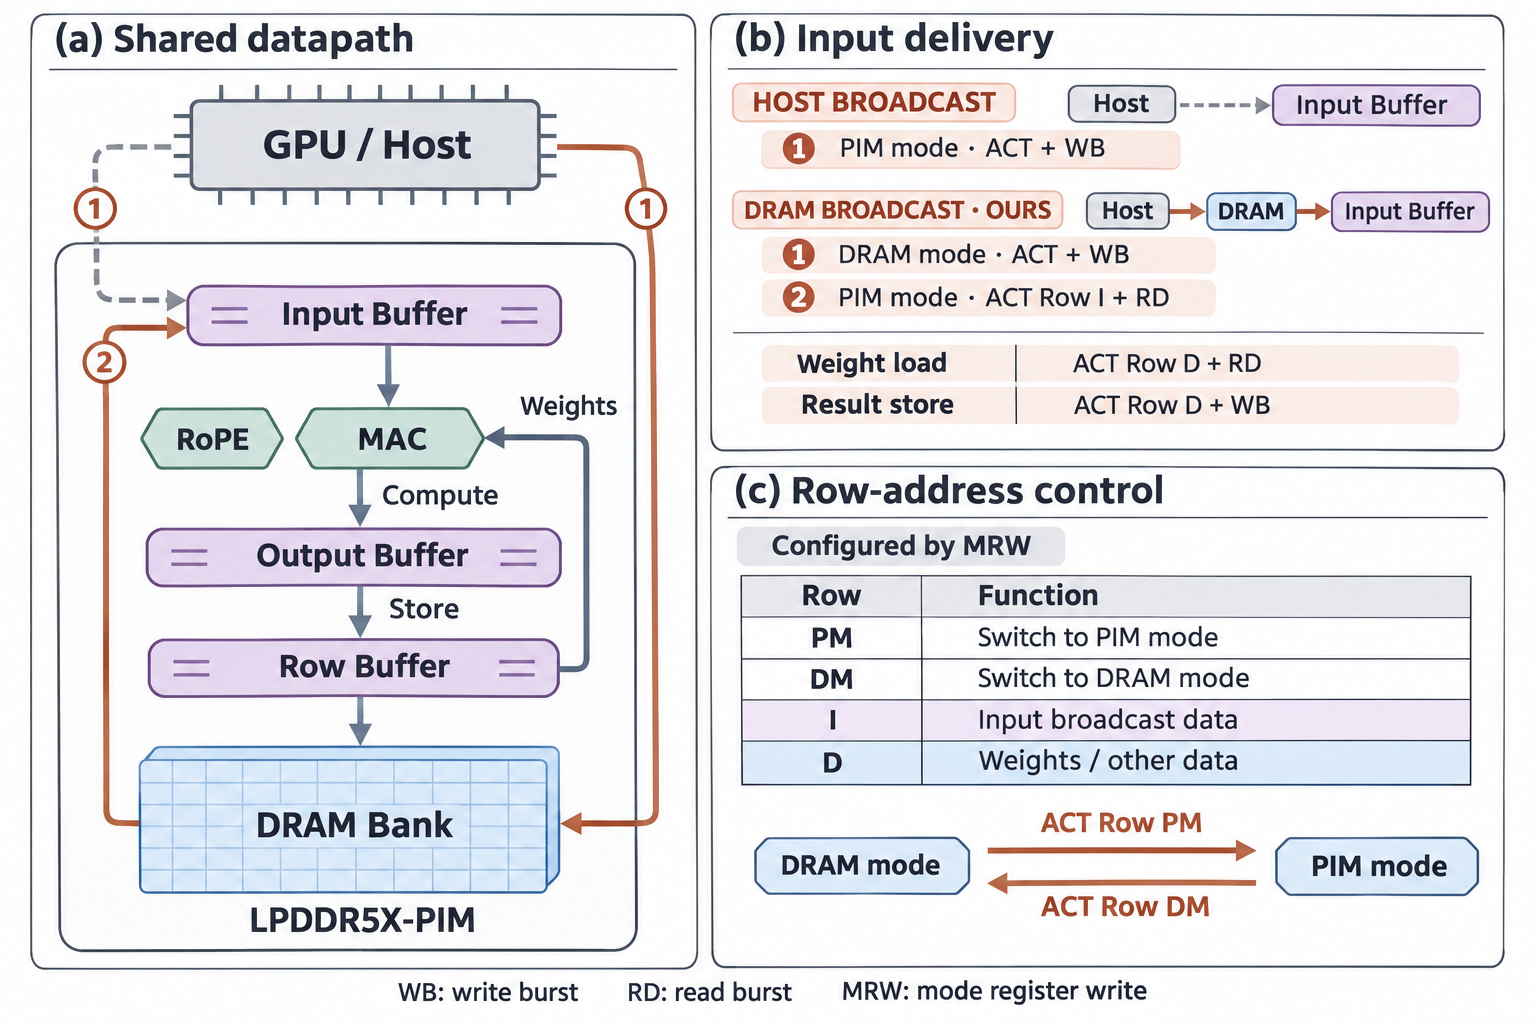
\includegraphics[width=0.82\textwidth]{figures/lpddr5x_pim_B_porcelain.png}
\caption{Input-preloading microarchitecture and function-row control. (a) Shared datapath; (b) host broadcast and in-DRAM broadcast; (c) function rows configured by MRW and mode switching.}
\label{fig:preload}
\end{figure*}

Existing designs such as LPDDR5X-PIM stream inputs from the host, so the DQ bus is intermittently occupied throughout the execution of an operator. This is unfriendly to the frequent rank switching in \sys{}. Either the WCKs of both ranks are kept synchronized at the cost of the power of an idling high-frequency data clock, or every switch pays the time of WCK synchronization and bus read/write (R/W) turnaround. Under JEDEC LPDDR5X-8533 timing, a PIM write followed by a GPU read and then another PIM write incurs a total DQ boundary overhead of 13~CK. Adding one 2-CK read burst, a gap of at least 15~CK is needed to insert a single GPU read. Ramulator simulation shows that, with streaming input, 52.9\% of the gaps between adjacent PIM data bursts are shorter than 15~CK (Fig.~\ref{fig:gap}(a)) and cannot be used to issue any GPU memory request. To exploit the remaining, longer gaps, the memory controller (MC) would additionally need DQ lookahead to predict whether each gap can accommodate the DQ burst of a GPU access, which complicates the arbitration logic.
% REVIEW (Alina Wong, gdoc comment c2 on the v3 draft): the "15 CK" threshold is disputed:
% "it should be at least 5 CK, and by probability the fraction is small". The same claim
% appears in Section V-B and in the Fig. gap caption. Resolve before submission.
\todo{Comment c2: the 15~CK threshold and the 52.9\% figure are disputed.}

\sys{} therefore uses a microarchitecture that suits rank partitioning better. Each bank gets an additional path from the Row Buffer to the Input Buffer, which supports an \emph{input-preloaded} dataflow (Fig.~\ref{fig:preload}):
\begin{enumerate}
\item \textbf{Bulk loading.} While the PIM rank is in DRAM mode, the host writes all inputs of an operator into the input region of the PIM rank (Row~I) at once and at full bandwidth, using ordinary WR commands.
\item \textbf{Local broadcast.} After the PIM rank switches to PIM mode, the MC issues an ACT to Row~I; the column data subsequently read out by RD are broadcast to the Input Buffers of all 16 banks.
\item \textbf{Local compute and write-back.} MAC results are written back to the result region in DRAM. After the computation, the host reads out all results at once in DRAM mode.
\end{enumerate}

This has two benefits. (a)~\textbf{DQ gap fusion.} Input transfers that were scattered across an operator are concentrated at its start. During PIM computation, the DQ bus is returned entirely to the GPU, which obtains long, contiguous access windows. (b)~\textbf{No fine-grained arbitration.} Since the inputs are ready in advance, the MC no longer needs DQ lookahead to decide whether a GPU command fits into a gap.

\textbf{C/A occupancy.} The linear operators of the AE are skinny GEMMs: a single RD column command completes the MAC for all $M$ input rows, so the command density is low. In simulation, the PIM rank occupies only 14.4\% of the external C/A cycles during PIM phases, and 54.4\% together with the C/A traffic of the GPU, so the C/A bus is not saturated. Preloading does not increase the C/A load either: with streaming input, the C/A occupancy of the PIM rank is 16.2\% (Section~\ref{sec:evaluation-b}).
% REVIEW (Alina Wong, gdoc comment c1 on the v3 draft): "This is odd, not what I meant to say.
% I recall running a simulation that replays the trace accounting for C/A occupancy, allowing
% 1-CK delays, etc." Rewrite this paragraph around that replay experiment.
\todo{Comment c1: rewrite this paragraph around the C/A-aware replay simulation.}

\subsection{PIM Command Interface and ISA Extension}
\label{sec:architecture-c}

\sys{} extends the JEDEC LPDDR5X command set with a PIM mode and defines the memory-side command-decoding state machine and ISA.

During LPDDR initialization, the host configures the function rows, including the mode-switch row and the input-buffer row, through Mode Register Writes (MRW). Afterwards, the MC only needs to activate the designated function row to switch a rank between DRAM mode and PIM mode.

In PIM mode, the same RD/WR is executed by all 16 banks in parallel, so the four address bits that normally select the bank group and the bank are unused. \sys{} uses these four bits to encode the operation type (Table~\ref{tab:isa}) and to specify which module writes its result back to DRAM \todo{microarchitecture figure}. All commands keep the JEDEC timing and pin semantics and are therefore compatible with a standard MC.

% Writing note from v3: the opcode table may be turned into a figure in the final version.
% Figure to be drawn: RD command format, marking the four reused BG/BA bits and the column-address bits.
% Local proposal v3; opcode assignments are unchanged.
\begin{table}[!t]
\caption{BG/BA Opcodes of RD/WR in PIM Mode}
\label{tab:isa}
\centering
\footnotesize
\setlength{\tabcolsep}{2.5pt}
\renewcommand{\arraystretch}{0.82}
\setlength{\aboverulesep}{1pt}
\setlength{\belowrulesep}{1pt}
\begin{tabularx}{\columnwidth}{@{}ccl>{\raggedright\arraybackslash}X@{}}
\toprule
\textbf{BG/BA} & \textbf{Cmd.} & \textbf{Operation} & \textbf{Function} \\
\midrule
0000 & RD & \texttt{MAC} & Accumulate MAC result \\
0001 & RD & \texttt{MAC\_INIT} & Initialize accumulator \\
0010 & RD & \texttt{MAC\_RED} & Multi-MAC reduction (reserved) \\
0011 & RD & \texttt{MAC\_INIT\_RED} & Single-MAC dot product + reduction \\
0100 & RD & \texttt{MAC\_INIT\_RED} & Dot/reduce; K BF16 lanes 0--7 \\
0101 & RD & \texttt{MAC\_INIT\_RED} & Dot/reduce; K BF16 lanes 8--15 \\
0110 & RD & \texttt{RD\_ROPE} & Load sin/cos into RoPE registers \\
0111 & RD & \texttt{RD\_ROPE\_Q} & Load and rotate Q \\
1000 & RD & \texttt{RD\_ROPE\_K} & Load and rotate K \\
\midrule
0000 & WR & \texttt{WB\_ACC} & Store accumulator to DRAM \\
0001 & WR & \texttt{WB\_MAC} & MAC bypass to DRAM (reserved) \\
0011 & WR & \texttt{WB\_OBUF} & Store output buffer to DRAM \\
\bottomrule
\end{tabularx}
\par\smallskip
\parbox{\columnwidth}{\scriptsize\mbox{\textit{RD Command:} \texttt{RD16}\,|\,\texttt{BG[1:0]}\,|\,\texttt{BA[1:0]}\,|\,Column Address \texttt{C[5:0]}\,|\,\texttt{AP}}}
\end{table}

